\chapter{Implementasi dan Pengujian Perangkat Lunak}
\label{chap:implementasidanpengujian}

Bab ini terdiri atas tiga bagian, yaitu Implementasi Perangkat Lunak, Implementasi Basis Data dan Pengujian Perangkat Lunak. Bagian implementasi berisi penjelasan lingkungan pengembangan perangkat lunak dan hasil implementasi perangkat lunak. Bagian implementasi basis data berisi penejelasan basis data yang telah diimplementasi, yang akan digunakan pada perangkat lunak. Sedangkan bagian pengujian berisi hasil pengujian terhadap perangkat lunak yang telah dibangun.

\section{Implementasi Perangkat Lunak}
\label{sec:implementasiperangkatlunak}

Pada bagian ini akan dibahas hasil implementasi perangkat lunak yang telah dibangun. Sub bab ini terdiri atas tiga bagian, yaitu lingkungan perangkat keras, lingkungan perangkat lunak, dan hasil implementasi perangkat lunak.

\subsection{Lingkungan Implementasi Perangkat Keras}
\label{sec:lingkunganimplementasiperangkatkeras}

Dalam membangun perangkat lunak ini digunakan spesifikasi perangkat keras sebagai berikut:

\begin{enumerate}
\item[(a)] Processor: AMD A10-5750M 2.5GHz
\item[(b)] RAM: 4 GB DDR3
\item[(c)] Harddisk: 1TB
\item[(d)] VGA: AMD Radeon HD 8650G 2GB
\item[(e)] Koneksi Internet: WAN
\end{enumerate}

\subsection{Lingkungan Implementasi Perangkat Lunak}
\label{sec:lingkunganimplementasiperangkatlunak}

Dalam membangun perangkat lunak ini digunakan spesifikasi perangkat lunak sebagai berikut:

\begin{enumerate}
\item[(a)] Sistem Operasi: Windows 8.1 Pro 64-bit
\item[(b)] Bahasa Pemrograman: PHP Version 5.6.3
\item[(c)] Aplikasi: XAMPP v5.6.3
\item[(d)] DBMS: MySQL
\item[(e)] Aplikasi Mesin Pencari: Google Chrome
\item[(f)] Library: Google APIs Client Library untuk PHP
\item[(g)] Javascript: Strapdown.js
\item[(h)] Framework: Foundation 5
\end{enumerate}

\subsection{Hasil Implementasi Perangkat Lunak}
\label{sec:hasilimplementasi}

Kode program perangkat lunak ditulis berdasarkan perancangan yang telah dibahas pada Bab~\ref{chap:perancangan}. Hasil implementasi perangkat lunak menghasilkan kode program berbasis PHP. Kode program yang telah diimplementasi dapat dilihat pada Lapiran~\ref{kode_program}.

\section{Implementasi Basis Data}
\label{sec:implementasibasisdata}

Implementasi basis data dalam sistem perekam dan berbagi riwayat mahasiswa, tahap pertama membuat sebuat basis data baru dan memberi nama spbrm untuk basis data tersebut. Untuk kode dapat dilihat di bawah ini.
\begin{lstlisting}[basicstyle=\footnotesize]
CREATE DATABASE 'spbrm' ;
\end{lstlisting}

Basis data sistem perekam dan berbagi riwayat mahasiswa menggunakan tiga tabel basis data. Tabel-tabel tersebut terdiri dari :
\begin{itemize}
\item Tabel InfoMahasiswa, digunakan untuk menyimpan semua data mahasiswa yang dapat diakses oleh pengguna. Untuk kode dapat dilihat di bawah ini.

\begin{lstlisting}[basicstyle=\footnotesize]
  CREATE TABLE 'info_mahasiswa' (
  'npm' varchar(10) NOT NULL,
  'nama' varchar(60) NOT NULL,
  'keterangan' text NOT NULL,
  'catatan' text NOT NULL,
  'pembaruan_terakhir' datetime NOT NULL DEFAULT CURRENT_TIMESTAMP,
  PRIMARY KEY ('npm'),
  ) ENGINE=InnoDB DEFAULT CHARSET=latin1 ;
\end{lstlisting}

\item Tabel Masalah, digunakan untuk menyimpan semua data masalah, antara lain masalah dengan siapa / mata kuliah apa dan masalahnya apa. Untuk kode dapat dilihat di bawah ini.

\begin{lstlisting}[basicstyle=\footnotesize]
  CREATE TABLE 'masalah' (
  'id_masalah' int(5) NOT NULL AUTO_INCREMENT,
  'npm' varchar(10) NOT NULL,
  'pengguna' varchar(60) NOT NULL,
  'masalah_dengan' varchar(25) NOT NULL,
  'masalah' text NOT NULL,
  'tanggal' datetime NOT NULL,
  PRIMARY KEY ('id_masalah'),
  KEY 'npm' ('npm'),
  ) ENGINE=InnoDB DEFAULT CHARSET=latin1 ;
\end{lstlisting}

\item Tabel Histori, digunakan untuk menyimpan semua data histori baik aksi pengguna dan riwayat mahasiswa. Untuk kode dapat dilihat di bawah ini.

\begin{lstlisting}[basicstyle=\footnotesize]
  CREATE TABLE 'histori' (
  'id_histori' int(5) NOT NULL AUTO_INCREMENT,
  'npm' varchar(10) NOT NULL,
  'pengguna' varchar(60) NOT NULL,
  'status' text NOT NULL,
  'tanggal_pembaruan' datetime NOT NULL,
  'keterangan' text NOT NULL,
  'catatan' text NOT NULL,
  PRIMARY KEY ('id_histori'),
  KEY 'npm' ('npm'),
  ) ENGINE=InnoDB DEFAULT CHARSET=latin1 ;
\end{lstlisting}
\end{itemize}

\section{Pengujian Perangkat Lunak}
\label{sec:pengujianperangkatlunak}

Pada bagian ini akan dibahas mengenai pengujian yang akan dilakukan terhadap perangkat lunak. Pengujian tersebut terdiri dari dua bagian yaitu pengujian fungsional dan pengujian eksperimental. Pengujian fungsional bertujuan untuk memastikan bahwa seluruh fungsi yang dibangun pada perangkat lunak berjalan sesuai dengan yang direncanakan. Sedangkan pengujian eksperimental bertujuan untuk mengujikan perangkat lunak langsung ke pengguna. Pada bagian pengujian untuk pengujian fungsional terdapat perubahan program pada bagian oauth.php, jadi dapat menjalankan pengujian dengan {\it email} yang diakhiri @student.unpar.ac.id dikarenakan penulis tidak memiliki {\it email} yang diakhiri @unpar.ac.id. Kode program untuk pengujian fungsional perangkat lunak dapat dilihat pada Lampiran \ref{kode_program_pengujian}.

\subsection{Lingkungan Pengujian Perangkat Keras}
\label{sec:lingkunganpengujianperangkatkeras}

Dalam pengujian perangkat lunak ini digunakan spesifikasi perangkat keras sebagai berikut:

\begin{enumerate}
\item[(a)] Processor: AMD A10-5750M 2.5GHz
\item[(b)] RAM: 4 GB DDR3
\item[(c)] Harddisk: 1TB
\item[(d)] VGA: AMD Radeon HD 8650G 2GB
\item[(e)] Koneksi Internet: WAN
\end{enumerate}

\subsection{Lingkungan Pengujian Perangkat Lunak}
\label{sec:lingkunganpengujianperangkatlunak}

Dalam pengujian perangkat lunak ini digunakan spesifikasi perangkat lunak sebagai berikut:

\begin{enumerate}
\item[(a)] Sistem Operasi: Windows 8.1 Pro 64-bit
\item[(b)] Bahasa Pemrograman: PHP Version 5.6.3
\item[(c)] Aplikasi: XAMPP v5.6.3
\item[(d)] DBMS: MySQL
\item[(e)] Aplikasi Mesin Pencari: Google Chrome
\item[(f)] Library: Google APIs Client Library untuk PHP
\item[(g)] Javascript: Strapdown.js
\item[(h)] Framework: Foundation 5
\end{enumerate}

\subsection{Pengujian Fungsional}
\label{sec:pengujianfungsional}
Pengujian fungsional menguji tampilan antar muka perangkat lunak beserta fungsi dasar. Berikut ini adalah daftar pengujian yang dilakukan:
\begin{enumerate}[(1)]
\item Fungsi login\\
    Pengujian fungsi ini dilakukan untuk memastikan perangkat lunak terhubung ke server Google untuk melakukan otentikasi dan otorisasi serta memeriksa apakah {\it email} yang digunakan untuk login diakhiri "@unpar.ac.id" atau "@student.unpar.ac.id" dikarenakan penulis tidak mempunyai akun dosen.
    
    Contoh kasus adalah melakukan login sebanyak dua kali, yang pertama menggunakan {\it email} yang diakhiri "@unpar.ac.id" atau "@student.unpar.ac.id", dan yang kedua menggunakan {\it email} yang diakhiri selain "@unpar.ac.id" dan "@student.unpar.ac.id". Pengujian pertama, pengguna membuka halaman index.php dapat dilihat pada Gambar \ref{fig:membukahalamanindex}. Lalu pengguna melakukan login menggunakan {\it email} "7310013@sudent.unpar.ac.id" dapat dilihat pada Gambar \ref{fig:logindenganstudent}. Lalu akan ada konfirmasi bahwa akun yang digunakan dikelola oleh student.unpar.ac.id dapat dilihat pada Gambar \ref{fig:konfirmasiemail}. Lalu pengguna akan diarahkan ke CAS (Central Authentication Service) UNPAR dan melakukan login kembali dapat dilihat pada Gambar \ref{fig:casunpar}. Lalu pengguna akan diminta untuk memberikan izin aksses dari pihak pengguna dapat dilihat pada Gambar \ref{fig:izindaripihakpengguna}. Setelah pengguna memberikan izin akses maka akan dilakukan dengan fungsi memilih mahasiswa yang akan dibahas pada poin berikutnya. Sedangkan pengujian kedua, pengguna melakukan login menggunakan {\it email} "bletack@gmail.com" dapat dilihat pada Gambar \ref{fig:logindengangmail}. Lalu pengguna akan mendapat {\it alert} karena {\it email} yang digunakan tidak sesuai dengan ketentuan dapat dilihat pada Gambar \ref{fig:alert}. Setelah pengguna menekan tombol ok pada {\it alert} maka pengguna akan dikembalikan ke halaman index.php. Hal ini menunjukkan fungsi login sudah berjalan dengan baik.

\item Fungsi memilih mahasiswa\\
	Pengujian fungsi ini dilakukan untuk memastikan pengguna dapat memilih mahasiswa. Pada halaman list.php terdapat tabel yang berisikan npm, nama, dan last update dan pengguna dapat memilih mahasiswa dengan menekan npm yang diinginkan. Contoh pengujian pengguna akan memilih mahasiswa dengan npm 2010730013 maka akan menghasilkan link yang mengarah ke $view.php?npm=2010730013$ dapat dilihat pada Gambar \ref{fig:memilihmahasiswa}. Hal ini menunjukkan fungsi memilih mahasiswa sudah berjalan dengan baik.
	
\item Fungsi mencari mahasiswa\\
    Pengujian fungsi ini dilakukan untuk memastikan pengguna dapat mencari mahasiswa yang ingin dicarinya. Pada halaman list.php terdapat tempat untuk memasukkan npm dari mahasiswa yang ingin dicari. Setelah memasukkan npm yang ingin dicari, kemudian pengguna menekan tombol "Cari NPM".
    
    Contoh kasus adalah melakukan pencarian mahasiswa dengan memasukkan npm seutuhnya dan sebagian npm. Pengujian pertama, pengguna memasukkan npm 2010730013 sebagai npm yang ingin dicari, dapat dilihat pada Gambar \ref{fig:mencarinpmutuh}. Kemudian pengguna menekan tombol "Cari NPM" sehingga pengguna mendapatkan hasil dari pencarian. Untuk hasil pencarian dapat dilihat pada Gambar \ref{fig:hasilmencarinpmutuh}. Pengujian kedua, pengguna memasukkan sebagian npm 2010 sebagai npm yang ingin dicari, dapat dilihat pada Gambar \ref{fig:mencarinpmsebagian}. Kemudian pengguna menekan tombol "Cari NPM" sehingga pengguna mendapatkan hasil dari pencarian. Untuk hasil pencarian dapat dilihat pada Gambar \ref{fig:hasilmencarinpmsebagian}.
	
\item Fungsi melihat info mahasiswa\\
	Pengujian fungsi ini dilakukan untuk memastikan pengguna dapat melihat informasi mahasiswa dari mahasiswa yang telah dipilih oleh pengguna. Contoh pengujian fungsi ini merupakan lanjutan dari fungsi memilih mahasiswa, dimana setelah pengguna memilih mahasiswa pada list.php maka sistem akan menampilkan informasi dari mahasiswa tersebut. Untuk gambar dapat dilihat pada Gambar \ref{fig:melihatinfomahasiswa}. Hal ini menunjukkan fungsi melihat info mahasiswa sudah berjalan dengan baik.
	
\item Fungsi mengedit info mahasiswa\\
	Pengujian fungsi ini dilakukan untuk memastikan informasi mahasiswa dapat diedit. Contoh pengujian mengambil informasi dari mahasiswa yang telah dilihat informasinya pada fungsi melihat info mahasiswa. Dimana keterangan sebagai salah satu informasi mahasiswa yang ada akan ditampilkan dan pengguna dapat melakukan perubahan lalu menyimpan perubahan dengan menekan tombol "Simpan". Untuk gambar dapat dilihat pada Gambar \ref{fig:mengeditinfomahasiswa}. Setelah menyimpan perubahan, pengguna akan dibawa kembali ke halaman list.php. Hal ini menunjukkan fungsi mengedit info mahasiswa sudah berjalan dengan baik.

\item Fungsi menambah masalah baru\\
    Pengujian fungsi ini dilakukan untuk memastikan pengguna dapat menambah masalah baru dari seorang mahasiswa. Contoh pengujian menambahkan masalah baru dari seorang mahasiswa dengan mengisikan form masalah baru, masalah dengan mata kuliah "AJK2" dan masalahnya "jarang mengikuti kelas praktikum dan jarang mengumpulkan tugas". Untuk gambar dapat dilihat pada Gambar \ref{fig:menambahmasalah}. Setelah menyimpan masalah baru, pengguna akan dibawa kembali ke halaman list.php. Hal ini menunjukkan fungsi menambah masalah baru sudah berjalan dengan baik.

\item Fungsi melihat daftar masalah\\
    Pengujian fungsi ini dilakukan untuk memastikan adanya daftar masalah dari seorang mahasiswa yang dipilih. Contoh pengujian melihat daftar masalah dari seorang mahasiswa yang memiliki npm 2010730013 dapat dilihat pada Gambar \ref{fig:melihatmasalah}. Hal ini menunjukkan fungsi melihat daftar masalah sudah berjalan dengan baik.

\item Fungsi melihat histori\\
	Pengujian fungsi ini dilakukan untuk memastikan adanya histori dari seorang mahasiswa yang dipilih dan dapat melihat versi keterangan yang pertama kali dibuat dan versi-versi berikutnya yang sudah dirubah. Contoh pengujian melihat histori dari seorang mahasiswa yang memiliki npm 2010730013 dapat dilihat pada Gambar \ref{fig:melihathistori} dan juga melihat keterangan versi pertama berserta versi berikutnya dapat dilihat pada Gambar \ref{fig:keteranganpertama} dan Gambar \ref{fig:keterangankedua}. Hal ini menunjukkan fungsi melihat histori sudah berjalan dengan baik.
	
\item Fungsi membuat entri baru\\
	Pengujian fungsi ini dilakukan untuk memastikan pada saat membuat entri baru terdapat format penulisan yang telah dibuat dengan Markdown dan berhasil menyimpan entri baru tersebut. Contoh pengujian menambahkan entri baru untuk mahasiswa yang memiliki npm "2010730005", nama "Grady Ireneus", deskripsi umum "Mahasiswa ini telah menyelesaikan setengah skripsi yang diambil. Sisanya akan diselesaikan semester depan" dan catatan "6 Juli 2015, Melakukan perwalian". Mengisi data npm, nama, deskripsi umum dan catatan sesuai penjabaran sebelumnya, untuk gambar dapat dilihat pada Gambar \ref{fig:membuatentribaru}. Setelah pengguna menekan tombol "Simpan" maka data yang telah dimasukkan akan tersimpan dan pengguna akan dikembalikan ke halaman list.php. Pengguna dapat melihat entri baru dengan npm 2010730005 dan nama Grady Ireneus telah masuk kedalam tabel dapat dilihat pada Gambar \ref{fig:entribaruberhasil}. Hal ini menunjukkan fungsi membuat entri baru sudah berjalan dengan baik.
	
\item Antarmuka yang responsif\\
    Pengujian antarmuka yang responsif dilakukan untuk memastikan tampilan antarmuka yang dibuat menggunakan Zurb Foundation berhasil. Contoh pengujian dilakukan dengan menggunakan mesin pencari yang telah dikecilkan ukurannya, lalu membuka index.php, list.php, dan new.php pada mesin pencari tersebut. Pengujian untuk index.php dapat dilihat pada Gambar \ref{fig:responsifindex}, untuk list.php dapat dilihat pada Gambar \ref{fig:responsiflist}, dan untuk new.php dapat dilihat pada Gambar \ref{fig:responsifnew}. Hal ini menunjukkan antarmuka yang responsif sudah berjalan dengan baik.
\end{enumerate}

\begin{figure}[H]
\centering
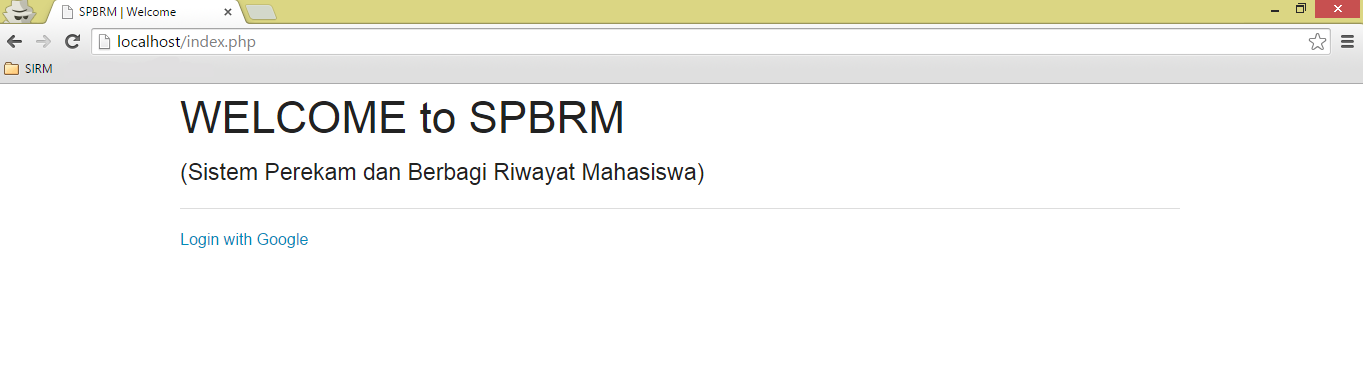
\includegraphics[scale=0.44]{Gambar/pengujian1.png}
\caption[Membuka Halaman index.php]{Membuka Halaman index.php} 
\label{fig:membukahalamanindex}
\end{figure}

\begin{figure}[H]
\centering
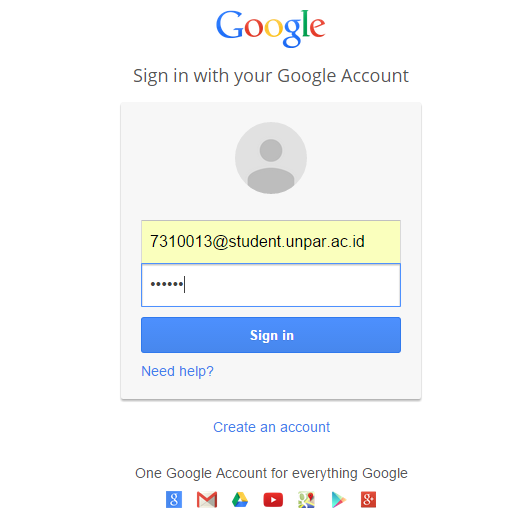
\includegraphics[scale=0.44]{Gambar/pengujian2.png}
\caption[Login Dengan {\it Email} yang Diakhiri "@student.unpar.ac.id"]{Login Dengan {\it Email} yang Diakhiri "@student.unpar.ac.id"}
\label{fig:logindenganstudent}
\end{figure}

\begin{figure}[H]
\centering
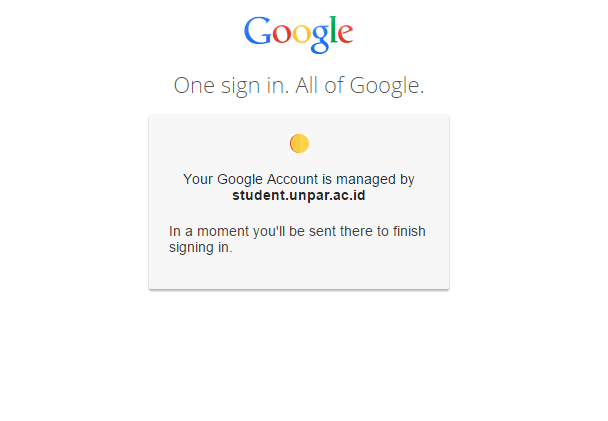
\includegraphics[scale=0.44]{Gambar/pengujian3.png}
\caption[Konfirmasi {\it Email} yang Dikelola oleh student.unpar.ac.id]{Konfirmasi {\it Email} yang Dikelola oleh student.unpar.ac.id}
\label{fig:konfirmasiemail}
\end{figure}

\begin{figure}[H]
\centering
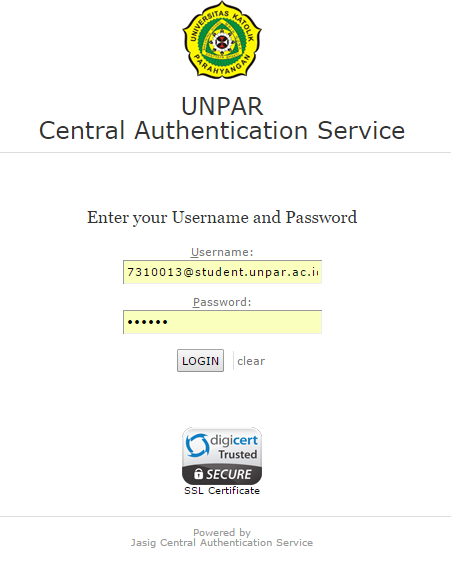
\includegraphics[scale=0.44]{Gambar/pengujian4.png}
\caption[CAS UNPAR]{CAS UNPAR} 
\label{fig:casunpar}
\end{figure}

\begin{figure}[H]
\centering
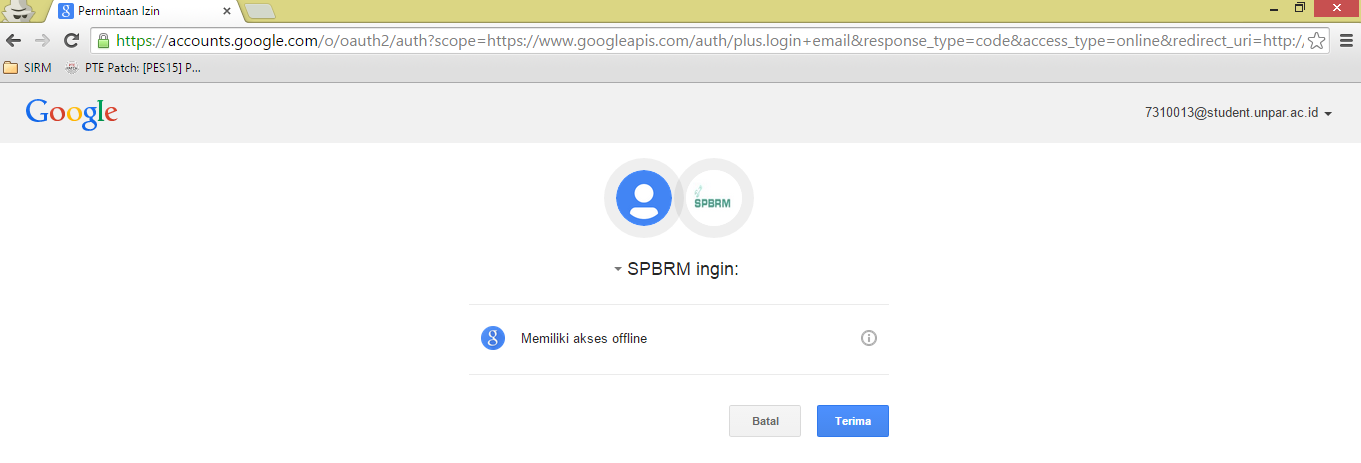
\includegraphics[scale=0.44]{Gambar/pengujian5.png}
\caption[Izin Akses Dari Pihak Pengguna]{Izin Akses Dari Pihak Pengguna} 
\label{fig:izindaripihakpengguna}
\end{figure}

\begin{figure}[H]
\centering
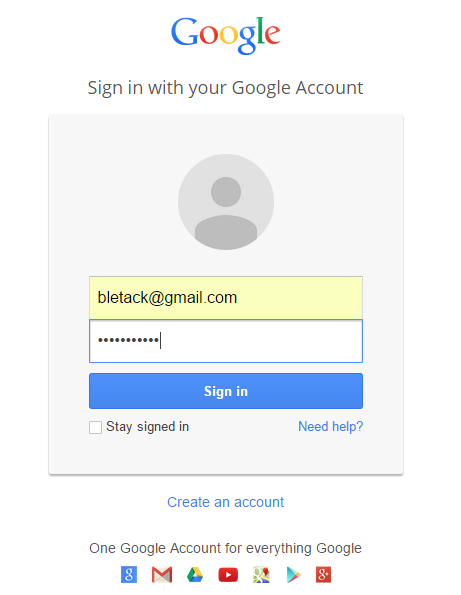
\includegraphics[scale=0.44]{Gambar/pengujian6.png}
\caption[Login Dengan {\it Email} yang Diakhiri "@gmail.com"]{Login Dengan {\it Email} yang Diakhiri "@gmail.com"}
\label{fig:logindengangmail}
\end{figure}

\begin{figure}[H]
\centering
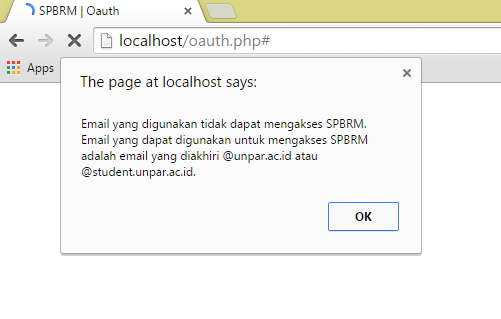
\includegraphics[scale=0.44]{Gambar/pengujian7.png}
\caption[Alert {\it Email} yang Digunakan Tidak Dapat Mengakses SPBRM]{Alert {\it Email} yang Digunakan Tidak Dapat Mengakses SPBRM}
\label{fig:alert}
\end{figure}

\begin{figure}[H]
\centering
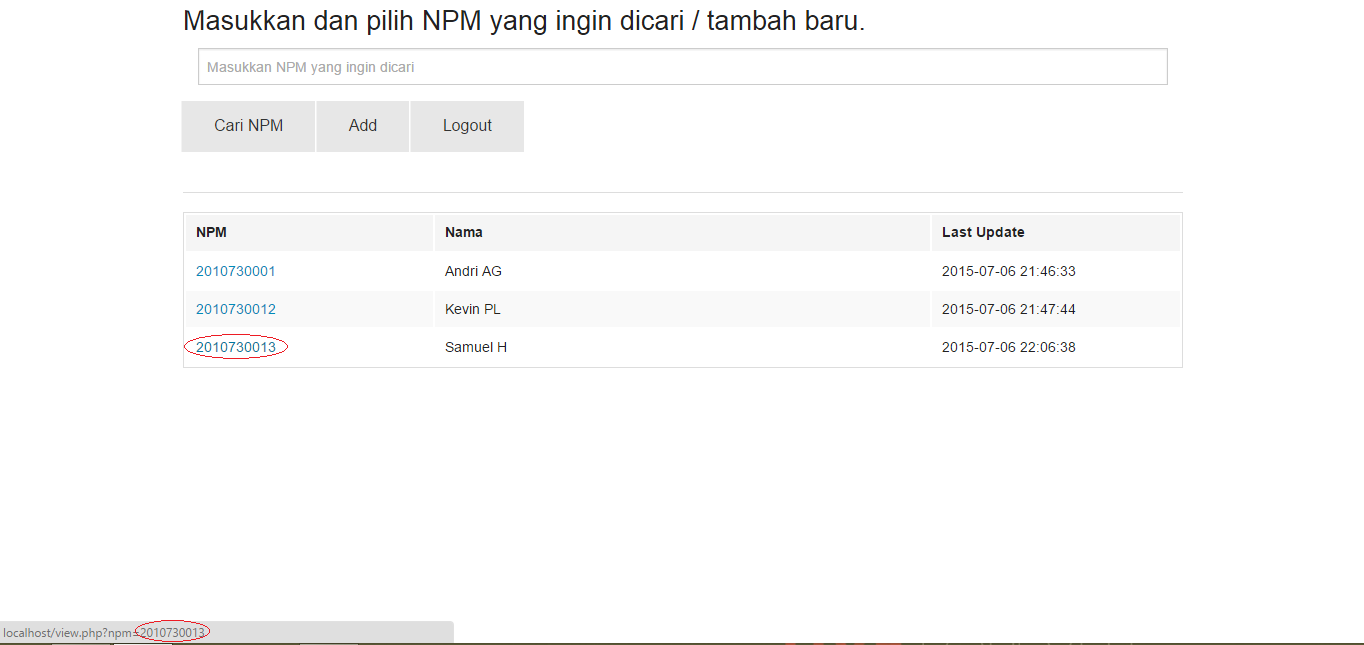
\includegraphics[scale=0.445]{Gambar/pengujian8.png}
\caption[Memilih Mahasiswa]{Memilih Mahasiswa} 
\label{fig:memilihmahasiswa}
\end{figure}

\begin{figure}[H]
\centering
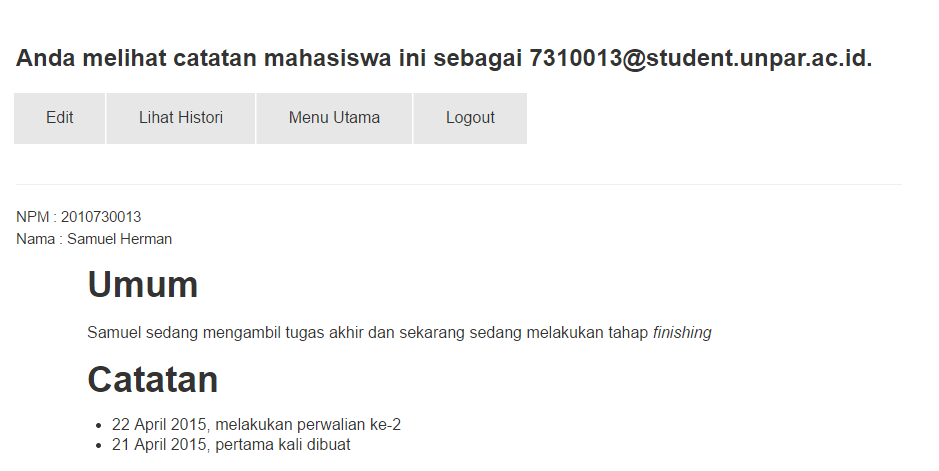
\includegraphics[scale=0.44]{Gambar/pengujian9.png}
\caption[Mencari Mahasiswa Dengan NPM Seutuhnya]{Mencari Mahasiswa Dengan NPM Seutuhnya} 
\label{fig:mencarinpmutuh}
\end{figure}

\begin{figure}[H]
\centering
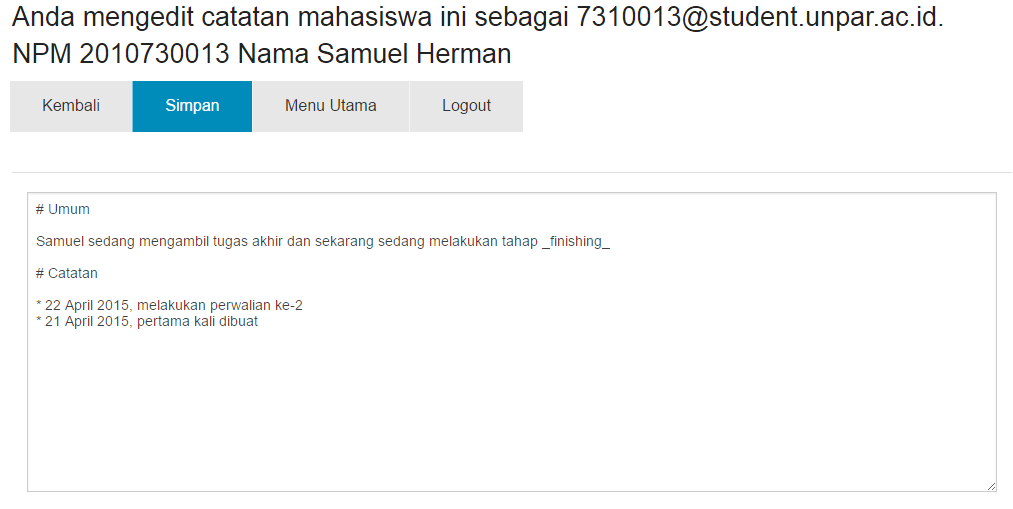
\includegraphics[scale=0.44]{Gambar/pengujian10.png}
\caption[Hasil Mencari Mahasiswa Dengan NPM Seutuhnya]{Hasil Mencari Mahasiswa Dengan NPM Seutuhnya}
\label{fig:hasilmencarinpmutuh}
\end{figure}

\begin{figure}[H]
\centering
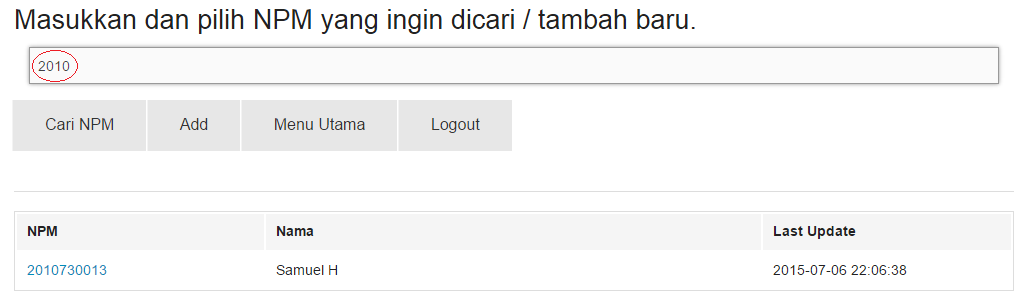
\includegraphics[scale=0.44]{Gambar/pengujian11.png}
\caption[Mencari Mahasiswa Dengan Sebagian NPM]{Mencari Mahasiswa Dengan Sebagian NPM} 
\label{fig:mencarinpmsebagian}
\end{figure}

\begin{figure}[H]
\centering
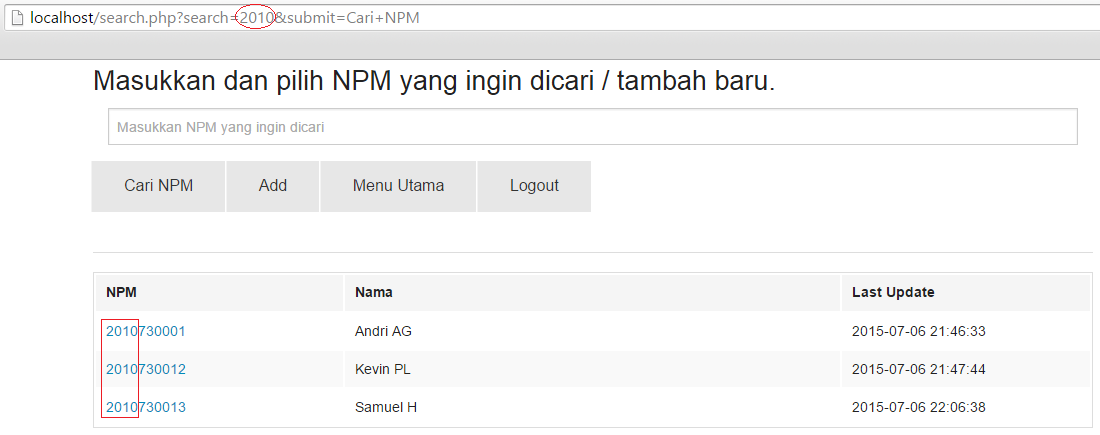
\includegraphics[scale=0.44]{Gambar/pengujian12.png}
\caption[Hasil Mencari Mahasiswa Dengan Sebagian NPM]{Hasil Mencari Mahasiswa Dengan Sebagian NPM}
\label{fig:hasilmencarinpmsebagian}
\end{figure}

\begin{figure}[H]
\centering
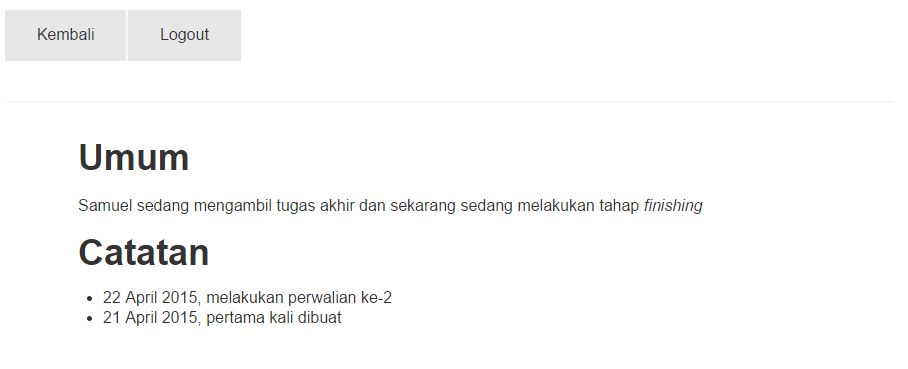
\includegraphics[scale=0.44]{Gambar/pengujian13.png}
\caption[Melihat Info Mahasiswa]{Melihat Info Mahasiswa} 
\label{fig:melihatinfomahasiswa}
\end{figure}

\begin{figure}[H]
\centering
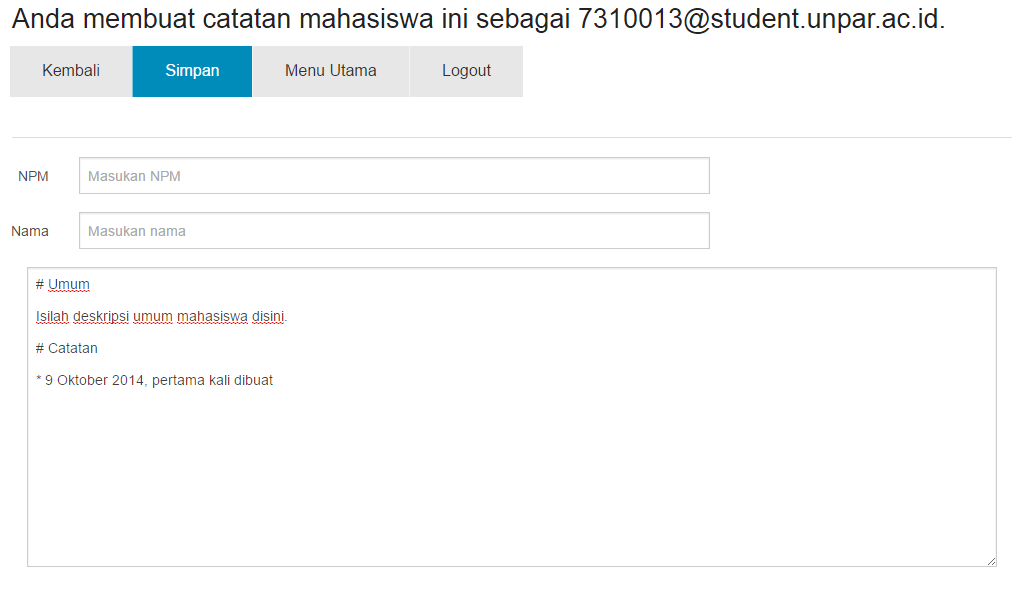
\includegraphics[scale=0.44]{Gambar/pengujian14.png}
\caption[Mengedit Info Mahasiswa]{Mengedit Info Mahasiswa} 
\label{fig:mengeditinfomahasiswa}
\end{figure}

\begin{figure}[H]
\centering
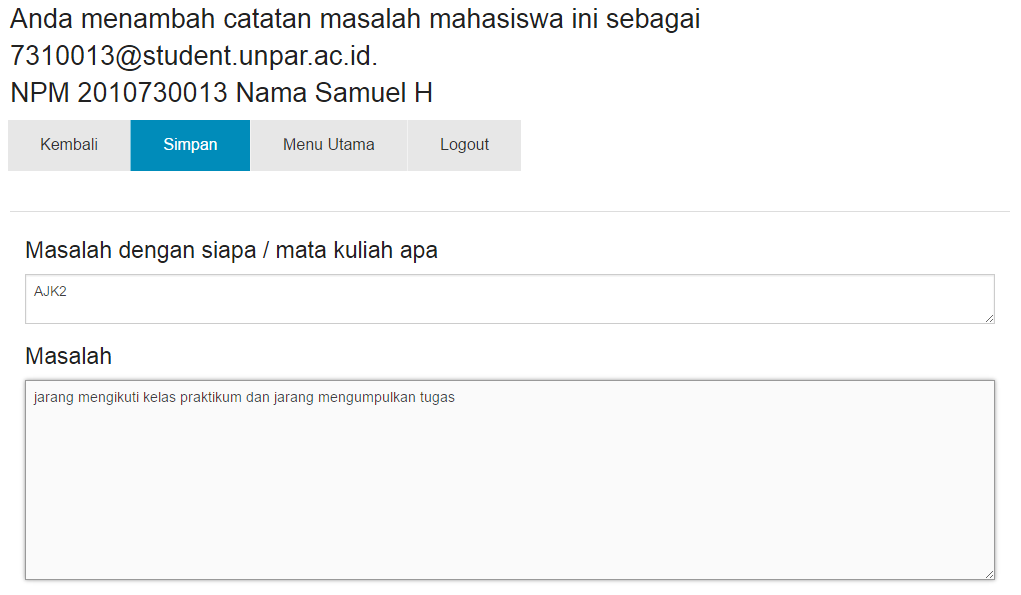
\includegraphics[scale=0.44]{Gambar/pengujian15.png}
\caption[Menambah Catatan Masalah Baru]{Menambah Catatan Masalah Baru} 
\label{fig:menambahmasalah}
\end{figure}

\begin{figure}[H]
\centering
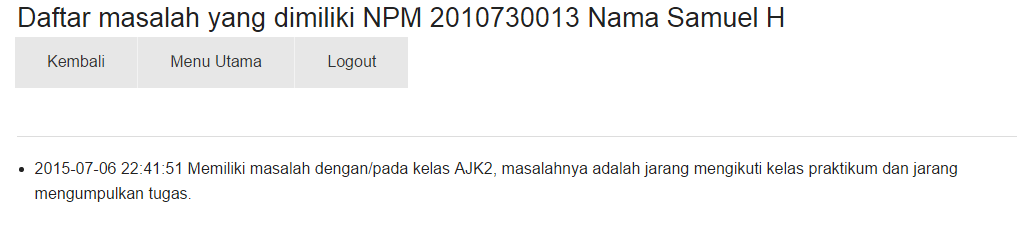
\includegraphics[scale=0.44]{Gambar/pengujian16.png}
\caption[Melihat Daftar Masalah]{Melihat Daftar Masalah} 
\label{fig:melihatmasalah}
\end{figure}

\begin{figure}[H]
\centering
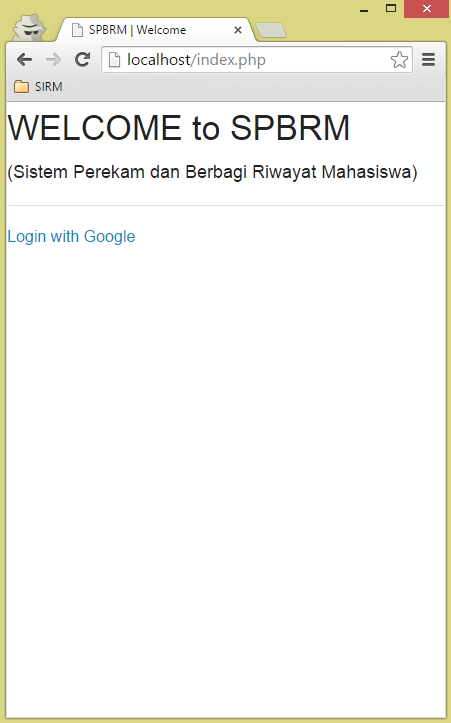
\includegraphics[scale=0.44]{Gambar/pengujian17.png}
\caption[Melihat Histori]{Melihat Histori} 
\label{fig:melihathistori}
\end{figure}

\begin{figure}[H]
\centering
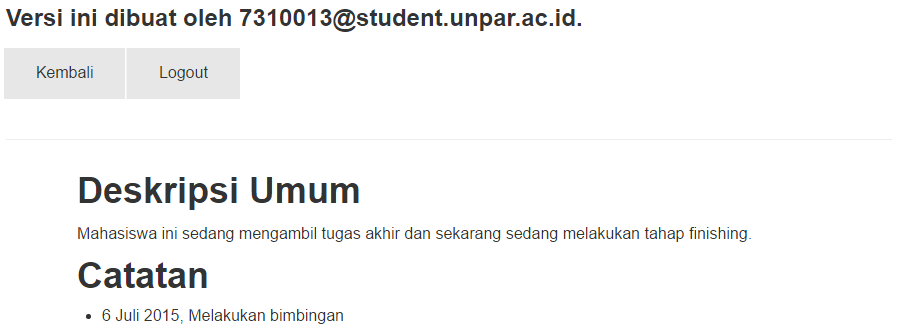
\includegraphics[scale=0.44]{Gambar/pengujian18.png}
\caption[Keterangan Versi Pertama]{Keterangan Versi Pertama} 
\label{fig:keteranganpertama}
\end{figure}

\begin{figure}[H]
\centering
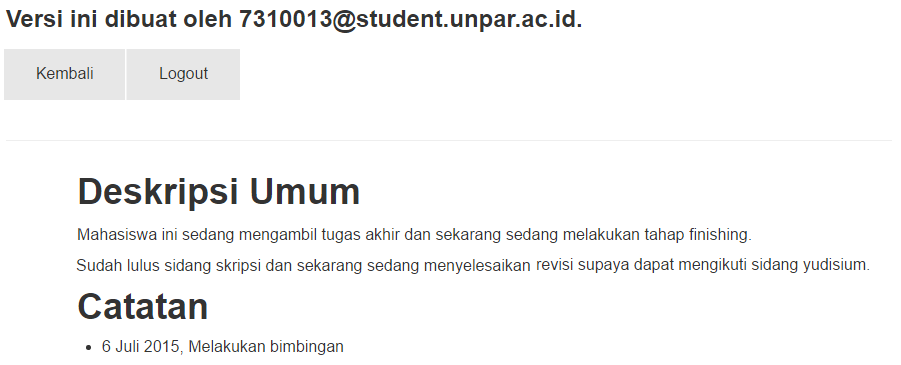
\includegraphics[scale=0.44]{Gambar/pengujian19.png}
\caption[Keterangan Versi Kedua]{Keterangan Versi Kedua} 
\label{fig:keterangankedua}
\end{figure}

\begin{figure}[H]
\centering
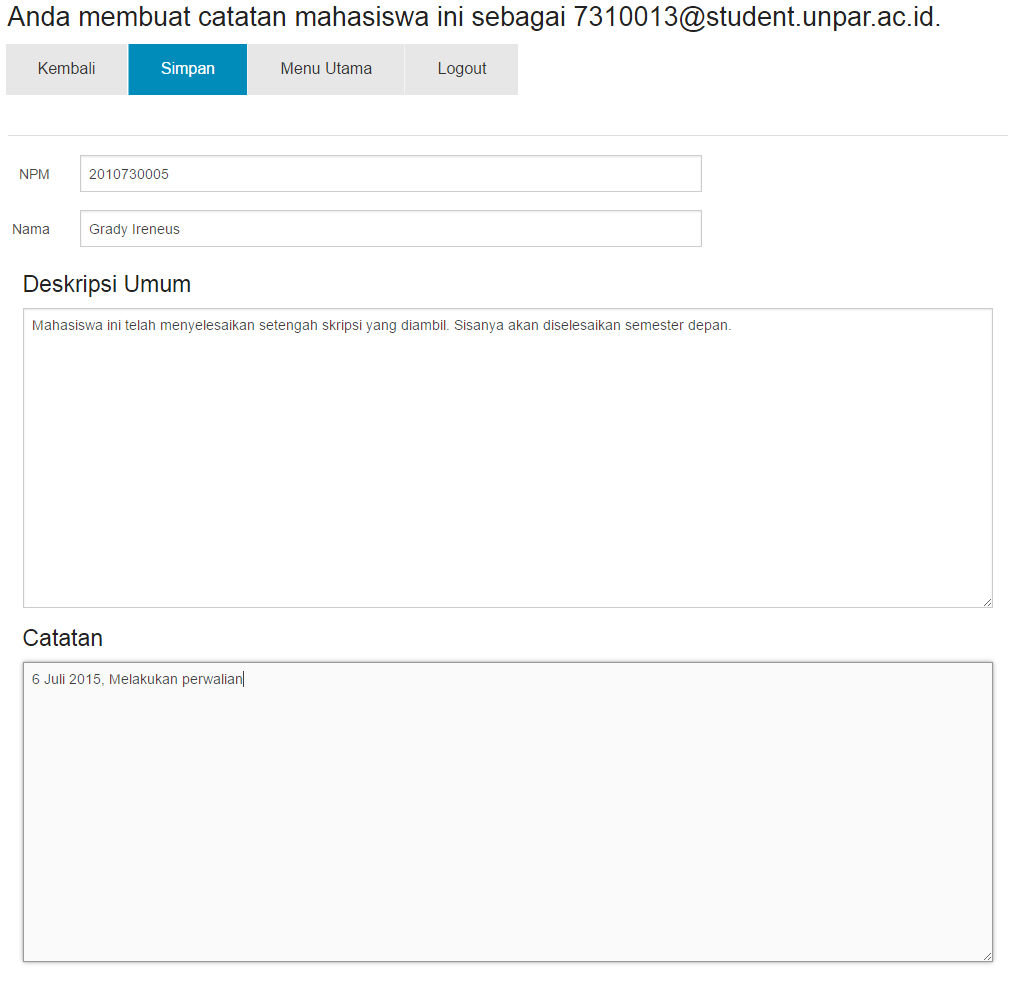
\includegraphics[scale=0.44]{Gambar/pengujian20.png}
\caption[Membuat Entri Baru]{Membuat Entri Baru} 
\label{fig:membuatentribaru}
\end{figure}

\begin{figure}[H]
\centering
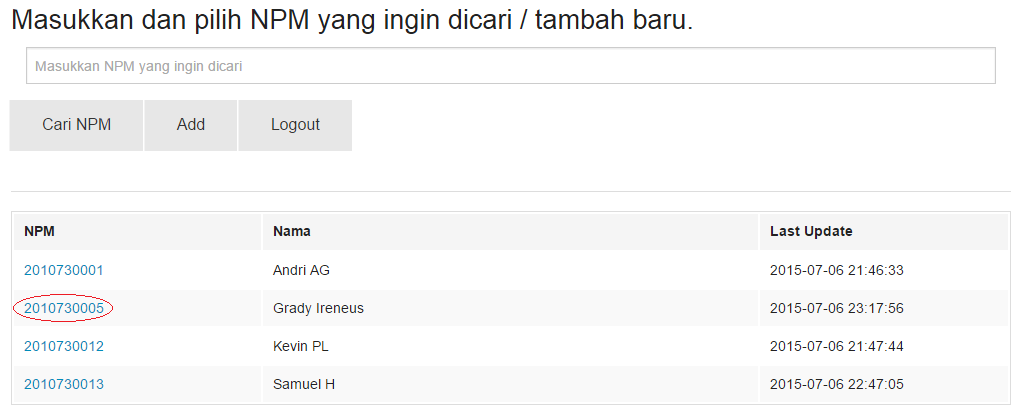
\includegraphics[scale=0.44]{Gambar/pengujian21.png}
\caption[Entri Baru Berhasil Dibuat]{Entri Baru Berhasil Dibuat} 
\label{fig:entribaruberhasil}
\end{figure}

\begin{figure}[H]
\centering
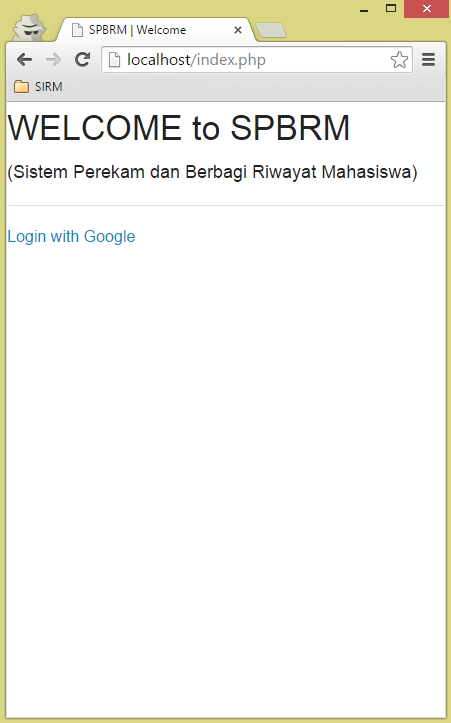
\includegraphics[scale=0.44]{Gambar/pengujian22.png}
\caption[Antarmuka Responsif index.php]{Antarmuka Responsif index.php} 
\label{fig:responsifindex}
\end{figure}

\begin{figure}[H]
\centering
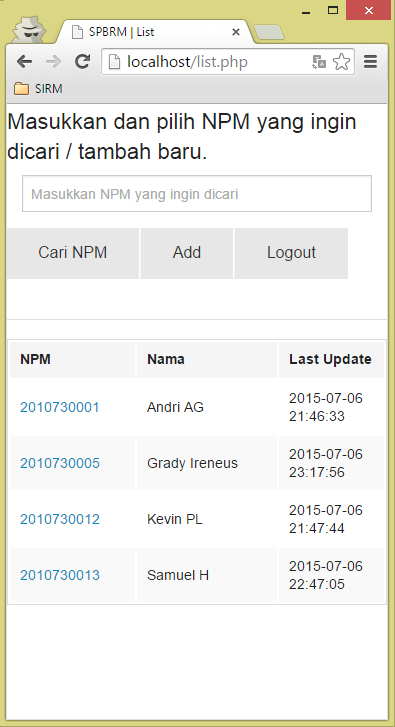
\includegraphics[scale=0.44]{Gambar/pengujian23.png}
\caption[Antarmuka Responsif list.php]{Antarmuka Responsif list.php} 
\label{fig:responsiflist}
\end{figure}

\begin{figure}[H]
\centering
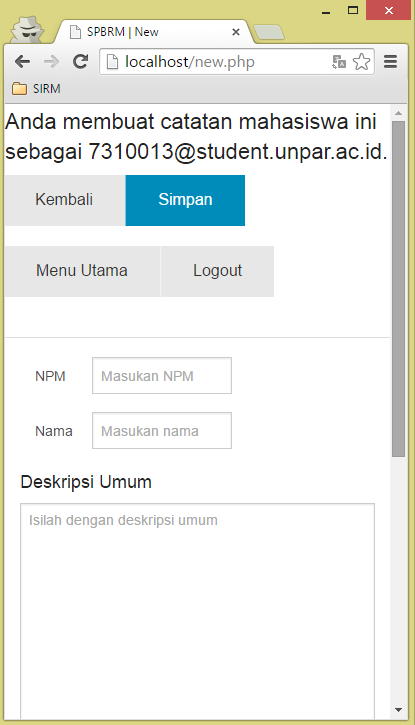
\includegraphics[scale=0.44]{Gambar/pengujian24.png}
\caption[Antarmuka Responsif new.php]{Antarmuka Responsif new.php} 
\label{fig:responsifnew}
\end{figure}

\subsection{Pengujian Eksperimental}
\label{sec:pengujianeksperimantal}

Pengujian eksperimental dilakukan langsung ke empat orang dosen Teknik Informatika. Keempat dosen menguji dengan cara mencoba semua fitur yang terdapat pada SPBRM. Keempat dosen juga menjalankan SPBRM dengan memasukkan data riwayat mahasiswa yang sebenarnya. Setelah melakukan pengujian diakhiri dengan kuesioner, untuk kuesioner pengujian eksperimental dapat dilihat pada Lampiran \ref{kuesionerpengujianeksperimental}. Untuk kuesioner dibuat menggunakan Google Form. Berikut data hasil kuesioner pengujian eksperimental, dapat dillihat pada Tabel \ref{kuesionerpertama}, \ref{kuesionerkedua}, \ref{kuesionerketiga}, \ref{kuesionerkeempat}, dan \ref{kuesionerkelima}.

\begin{table}[H]
\centering
\caption{Tabel Jawaban Pertanyaan Pertama, SPBRM Membantu Mengingat}
\label{kuesionerpertama}
\begin{tabular}{|l|l|l|l|l|l|}
\hline
No Penguji & Sangat Setuju & Setuju & Netral & Tidak Setuju & Sangat Tidak Setuju \\ \hline
1 & & \checkmark & & & \\ \hline
2 & \checkmark & & & & \\ \hline
3 & & \checkmark & & & \\ \hline
4 & & \checkmark & & & \\ \hline
\end{tabular}
\end{table}

\begin{table}[H]
\centering
\caption{Tabel Jawaban Pertanyaan Kedua, Kemudahan SPBRM}
\label{kuesionerkedua}
\begin{tabular}{|l|l|l|l|l|l|}
\hline
No Penguji & Sangat Setuju & Setuju & Netral & Tidak Setuju & Sangat Tidak Setuju \\ \hline
1 & & & \checkmark & & \\ \hline
2 & \checkmark & & & & \\ \hline
3 & & \checkmark & & & \\ \hline
4 & & \checkmark & & & \\ \hline
\end{tabular}
\end{table}

\begin{table}[H]
\centering
\caption{Tabel Jawaban Pertanyaan Ketiga, SPBRM Membantu Pemahaman}
\label{kuesionerketiga}
\begin{tabular}{|l|l|l|l|l|l|}
\hline
No Penguji & Sangat Setuju & Setuju & Netral & Tidak Setuju & Sangat Tidak Setuju \\ \hline
1 & & \checkmark & & & \\ \hline
2 & \checkmark & & & & \\ \hline
3 & & & & \checkmark & \\ \hline
4 & & \checkmark & & & \\ \hline
\end{tabular}
\end{table}

\begin{table}[H]
\centering
\caption{Tabel Jawaban Pertanyaan Keempat, SPBRM Efektif}
\label{kuesionerkeempat}
\begin{tabular}{|l|l|l|l|l|l|}
\hline
No Penguji & Sangat Setuju & Setuju & Netral & Tidak Setuju & Sangat Tidak Setuju \\ \hline
1 & & \checkmark & & & \\ \hline
2 & \checkmark & & & & \\ \hline
3 & & & & \checkmark & \\ \hline
4 & & & \checkmark & & \\ \hline
\end{tabular}
\end{table}

\begin{table}[H]
\centering
\caption{Tabel Jawaban Pertanyaan Kelima, SPBRM Efisien}
\label{kuesionerkelima}
\begin{tabular}{|l|l|l|l|l|l|}
\hline
No Penguji & Sangat Setuju & Setuju & Netral & Tidak Setuju & Sangat Tidak Setuju \\ \hline
1 & & \checkmark & & & \\ \hline
2 & \checkmark & & & & \\ \hline
3 & & & & \checkmark & \\ \hline
4 & & & \checkmark & & \\ \hline
\end{tabular}
\end{table}

\newcommand{\slice}[4]{
  \pgfmathparse{0.5*#1+0.5*#2}
  \let\midangle\pgfmathresult

  % slice
  \draw[thick,fill=black!10] (0,0) -- (#1:1) arc (#1:#2:1) -- cycle;

  % outer label
  \node[label=\midangle:#4] at (\midangle:1) {};

  % inner label
  \pgfmathparse{min((#2-#1-10)/110*(-0.3),0)}
  \let\temp\pgfmathresult
  \pgfmathparse{max(\temp,-0.5) + 0.8}
  \let\innerpos\pgfmathresult
  \node at (\midangle:\innerpos) {#3};
}

\begin{figure}
\centering
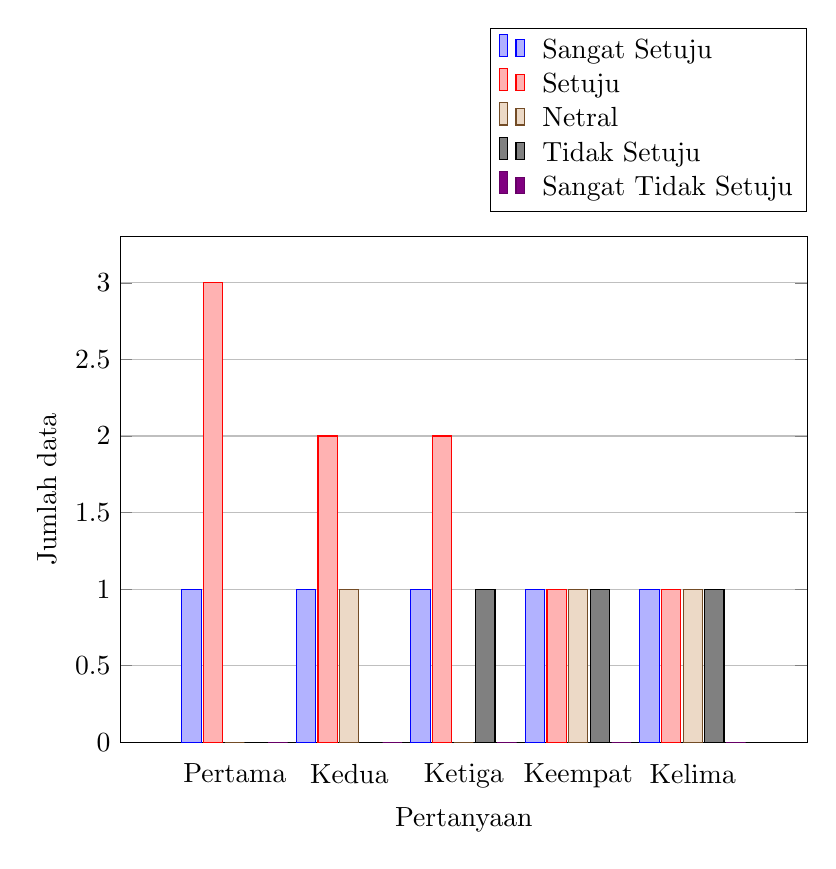
\begin{tikzpicture}
    \begin{axis}[
        width  = 0.85*\textwidth,
        height = 8cm,
        major x tick style = transparent,
        ybar=2*\pgflinewidth,
        bar width=7pt,
        ymajorgrids = true,
        ylabel = {Jumlah data},
        xlabel = {Pertanyaan},
        symbolic x coords={Pertama, Kedua, Ketiga, Keempat, Kelima},
        xtick = data,
        scaled y ticks = false,
        enlarge x limits=0.25,
        ymin=0,
        legend cell align=left,
        legend style={
                at={(1,1.05)},
                anchor=south east,
                column sep=1ex
        }
    ]
        \addplot
            coordinates {(Pertama, 1)(Kedua, 1)(Ketiga, 1)(Keempat, 1)(Kelima, 1)};

        \addplot
             coordinates {(Pertama, 3)(Kedua, 2)(Ketiga, 2)(Keempat, 1)(Kelima, 1)};

        \addplot
             coordinates {(Pertama, 0)(Kedua, 1)(Ketiga, 0)(Keempat, 1)(Kelima, 1)};

        \addplot
             coordinates {(Pertama, 0)(Kedua, 0)(Ketiga, 1)(Keempat, 1)(Kelima, 1)};
        
        \addplot
             coordinates {(Pertama, 0)(Kedua, 0)(Ketiga, 0)(Keempat, 0)(Kelima, 0)};

        \legend{Sangat Setuju,Setuju,Netral,Tidak Setuju,Sangat Tidak Setuju}
    \end{axis}
\end{tikzpicture}
\caption[Diagram Data Kuesioner]{Diagram Data Kuesioner}
\label{fig:diagramdatakuesioner}
\end{figure}

Berdasarkan Gambar \ref{fig:diagramdatakuesioner}, membuktikan beberapa hal sebagai berikut.
\begin{itemize}
\item Penguji setuju bahwa SPBRM membantu dalam mengingat setiap riwayat mahasiswa.
\item Penguji setuju bahwa SPBRM mudah untuk digunakan.
\item Penguji setuju bahwa SPBRM membantu pemahaman dalam mengelola riwayat mahasiswa. Namun terdapat responden yang menjawab tidak setuju, hal ini menjadi masukkan untuk pengembangan perangkat lunak. Sehingga semua pengguna benar-benar paham untuk mengelola riwayat mahasiswa menggunakan SPBRM.
\item Keempat penguji memberikan jawaban yang berbeda-beda untuk pertanyaan bekerja dengan SPBRM menjadi efektif dan efisien, sehingga menunjukkan adanya kebutuhan untuk meningkatkan aspek efektif dan efisien. Hal ini menjadi masukkan untuk pengembangan perangkat lunak sehingga semua pengguna yang bekerja dengan SPBRM dapat merasa efektif dan efisien.
\end{itemize}